\documentclass[aspectratio=169]{beamer}
\usetheme{metropolis}
\usepackage{graphicx}
\usepackage{booktabs}
\usepackage{hyperref}

% Colors
\definecolor{mDarkTeal}{HTML}{23373B}
\definecolor{mLightBrown}{HTML}{EB811B}

% Title info
\title{The Hero in Four Worlds}
\subtitle{AI-Powered Visual Storytelling}
\author{Student Name}
\institute{Graphics Processing Systems\\Politehnica University of Timișoara}
\date{January 2026}

\begin{document}

% ============================================
% SLIDE 1: Title
% ============================================
\begin{frame}
\titlepage
\end{frame}

% ============================================
% SLIDE 2: Introduction & Theme
% ============================================
\begin{frame}{Introduction \& Theme}
\begin{columns}
\column{0.5\textwidth}
\textbf{The Concept:}
\begin{itemize}
    \item One consistent hero character
    \item Four distinct world environments
    \item AI-powered image generation \& editing
\end{itemize}

\vspace{0.5cm}
\textbf{The Worlds:}
\begin{enumerate}
    \item Jungle — Origin story
    \item Medieval — Knight champion
    \item Desert — Journey continues
    \item Cyberpunk — Future memories
\end{enumerate}

\column{0.5\textwidth}
\begin{center}
\includegraphics[width=0.9\textwidth]{images/hero_reference.png}
\end{center}
\end{columns}
\end{frame}

% ============================================
% SLIDE 3: Tools Used
% ============================================
\begin{frame}{AI Tools Used}
\begin{columns}
\column{0.33\textwidth}
\begin{block}{Seedream 4.5}
\centering
Landscape generation\\
\textbf{Rating: 5/5}\\
\small Best quality, consistency
\end{block}

\column{0.33\textwidth}
\begin{block}{Nano Banana}
\centering
Character compositing\\
\textbf{Rating: 3/5}\\
\small Good positioning, quality drop
\end{block}

\column{0.33\textwidth}
\begin{block}{Flux-2 Pro}
\centering
In-context editing\\
\textbf{Rating: 5/5}\\
\small Best for creative edits
\end{block}
\end{columns}

\vspace{0.5cm}
\textbf{Workflow:} Seedream (backgrounds) $\rightarrow$ Nano Banana (insert hero) $\rightarrow$ Flux-2 (polish/edit)
\end{frame}

% ============================================
% SLIDE 4: Hero Character
% ============================================
\begin{frame}{The Hero Character}
\begin{columns}
\column{0.5\textwidth}
\textbf{Key Features:}
\begin{itemize}
    \item Sharp jawline, high cheekbones
    \item Hazel-green eyes, short goatee
    \item Dark slicked-back hair
    \item \textbf{Tattoo} on right forehand
    \item \textbf{Black ring} on left index finger
\end{itemize}

\vspace{0.3cm}
\textbf{Inspiration:} Timothée Chalamet (Dune)

\vspace{0.3cm}
\textbf{Consistency Challenge:}\\
Maintaining identity across 4 worlds + edits

\column{0.5\textwidth}
\begin{center}
\includegraphics[width=0.95\textwidth]{images/hero_reference.png}
\end{center}
\end{columns}
\end{frame}

% ============================================
% SLIDE 5: Jungle World
% ============================================
\begin{frame}{World 1: Jungle — Origin}
\begin{columns}
\column{0.6\textwidth}
\begin{center}
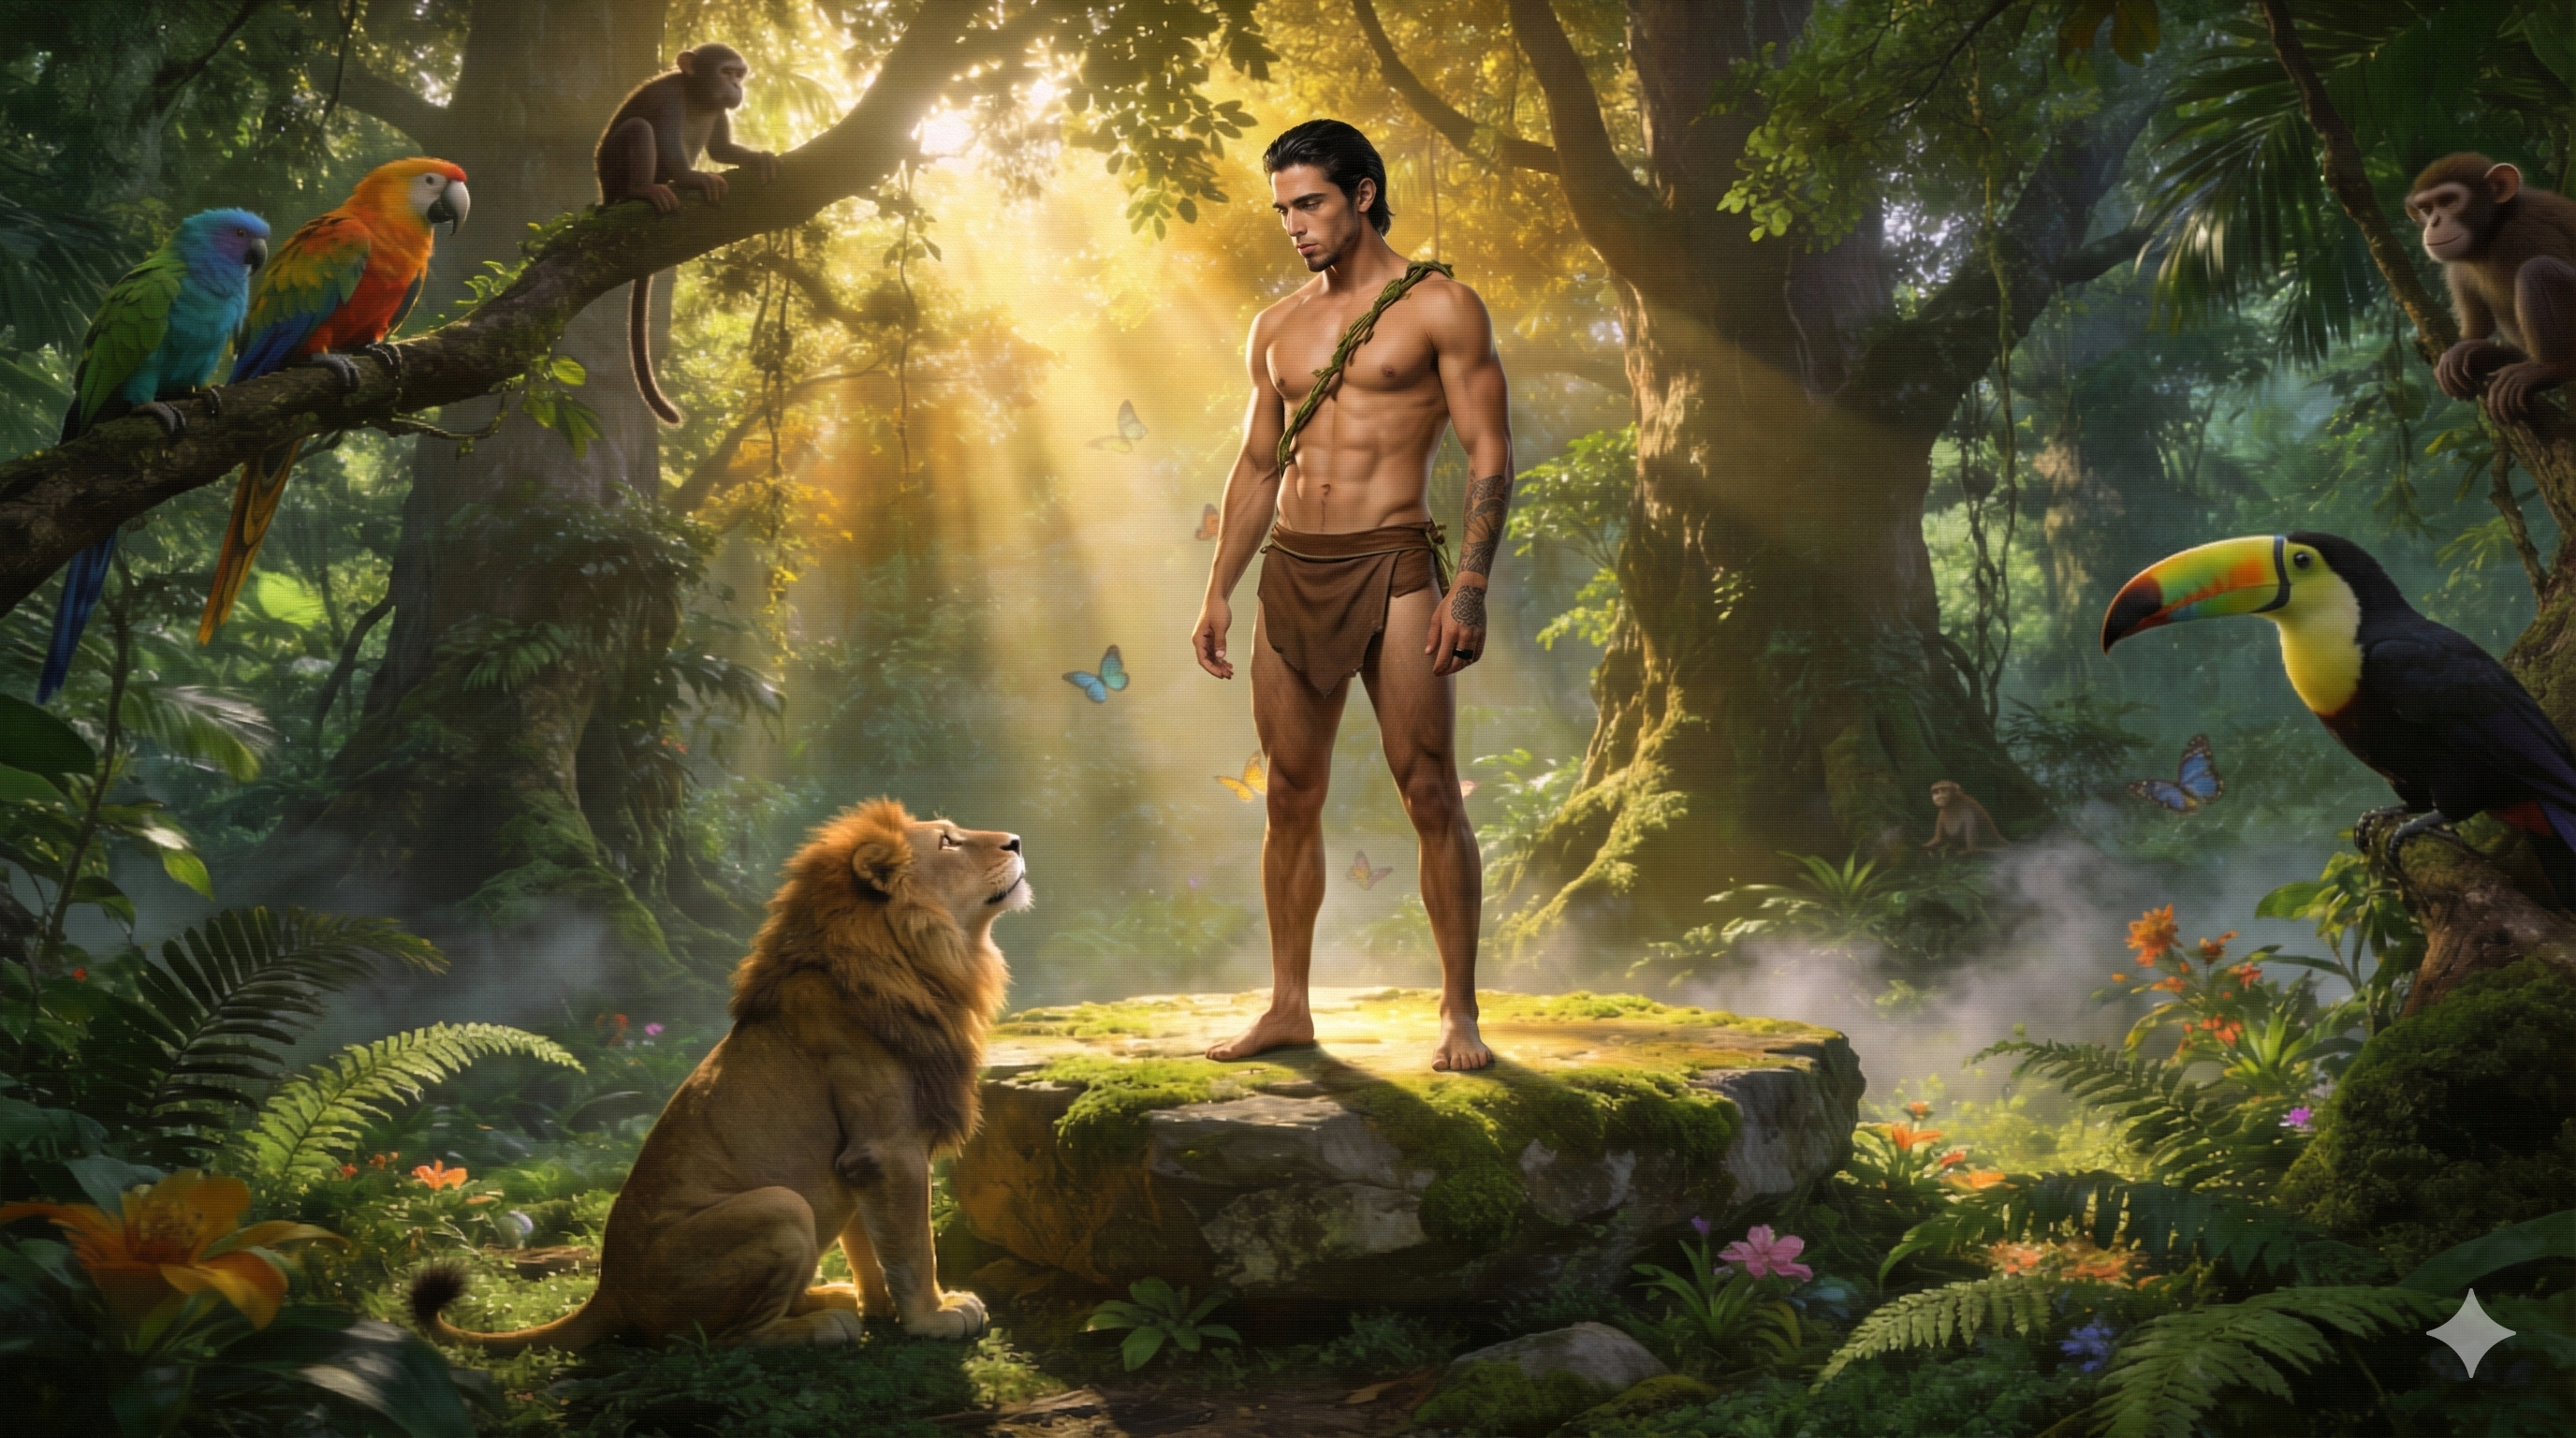
\includegraphics[width=\textwidth]{images/hero_in_backgrounds/jungle.png}
\end{center}

\column{0.4\textwidth}
\textbf{Story:} The hero receives a mystical ring from ancient spirits.

\vspace{0.3cm}
\textbf{Outfit:} Mowgli/Tarzan style

\vspace{0.3cm}
\textbf{Tools:}
\begin{itemize}
    \item Seedream: Background
    \item Nano Banana: Hero insert
\end{itemize}
\end{columns}
\end{frame}

% ============================================
% SLIDE 6: Medieval World
% ============================================
\begin{frame}{World 2: Medieval — Knight Champion}
\begin{columns}
\column{0.6\textwidth}
\begin{center}
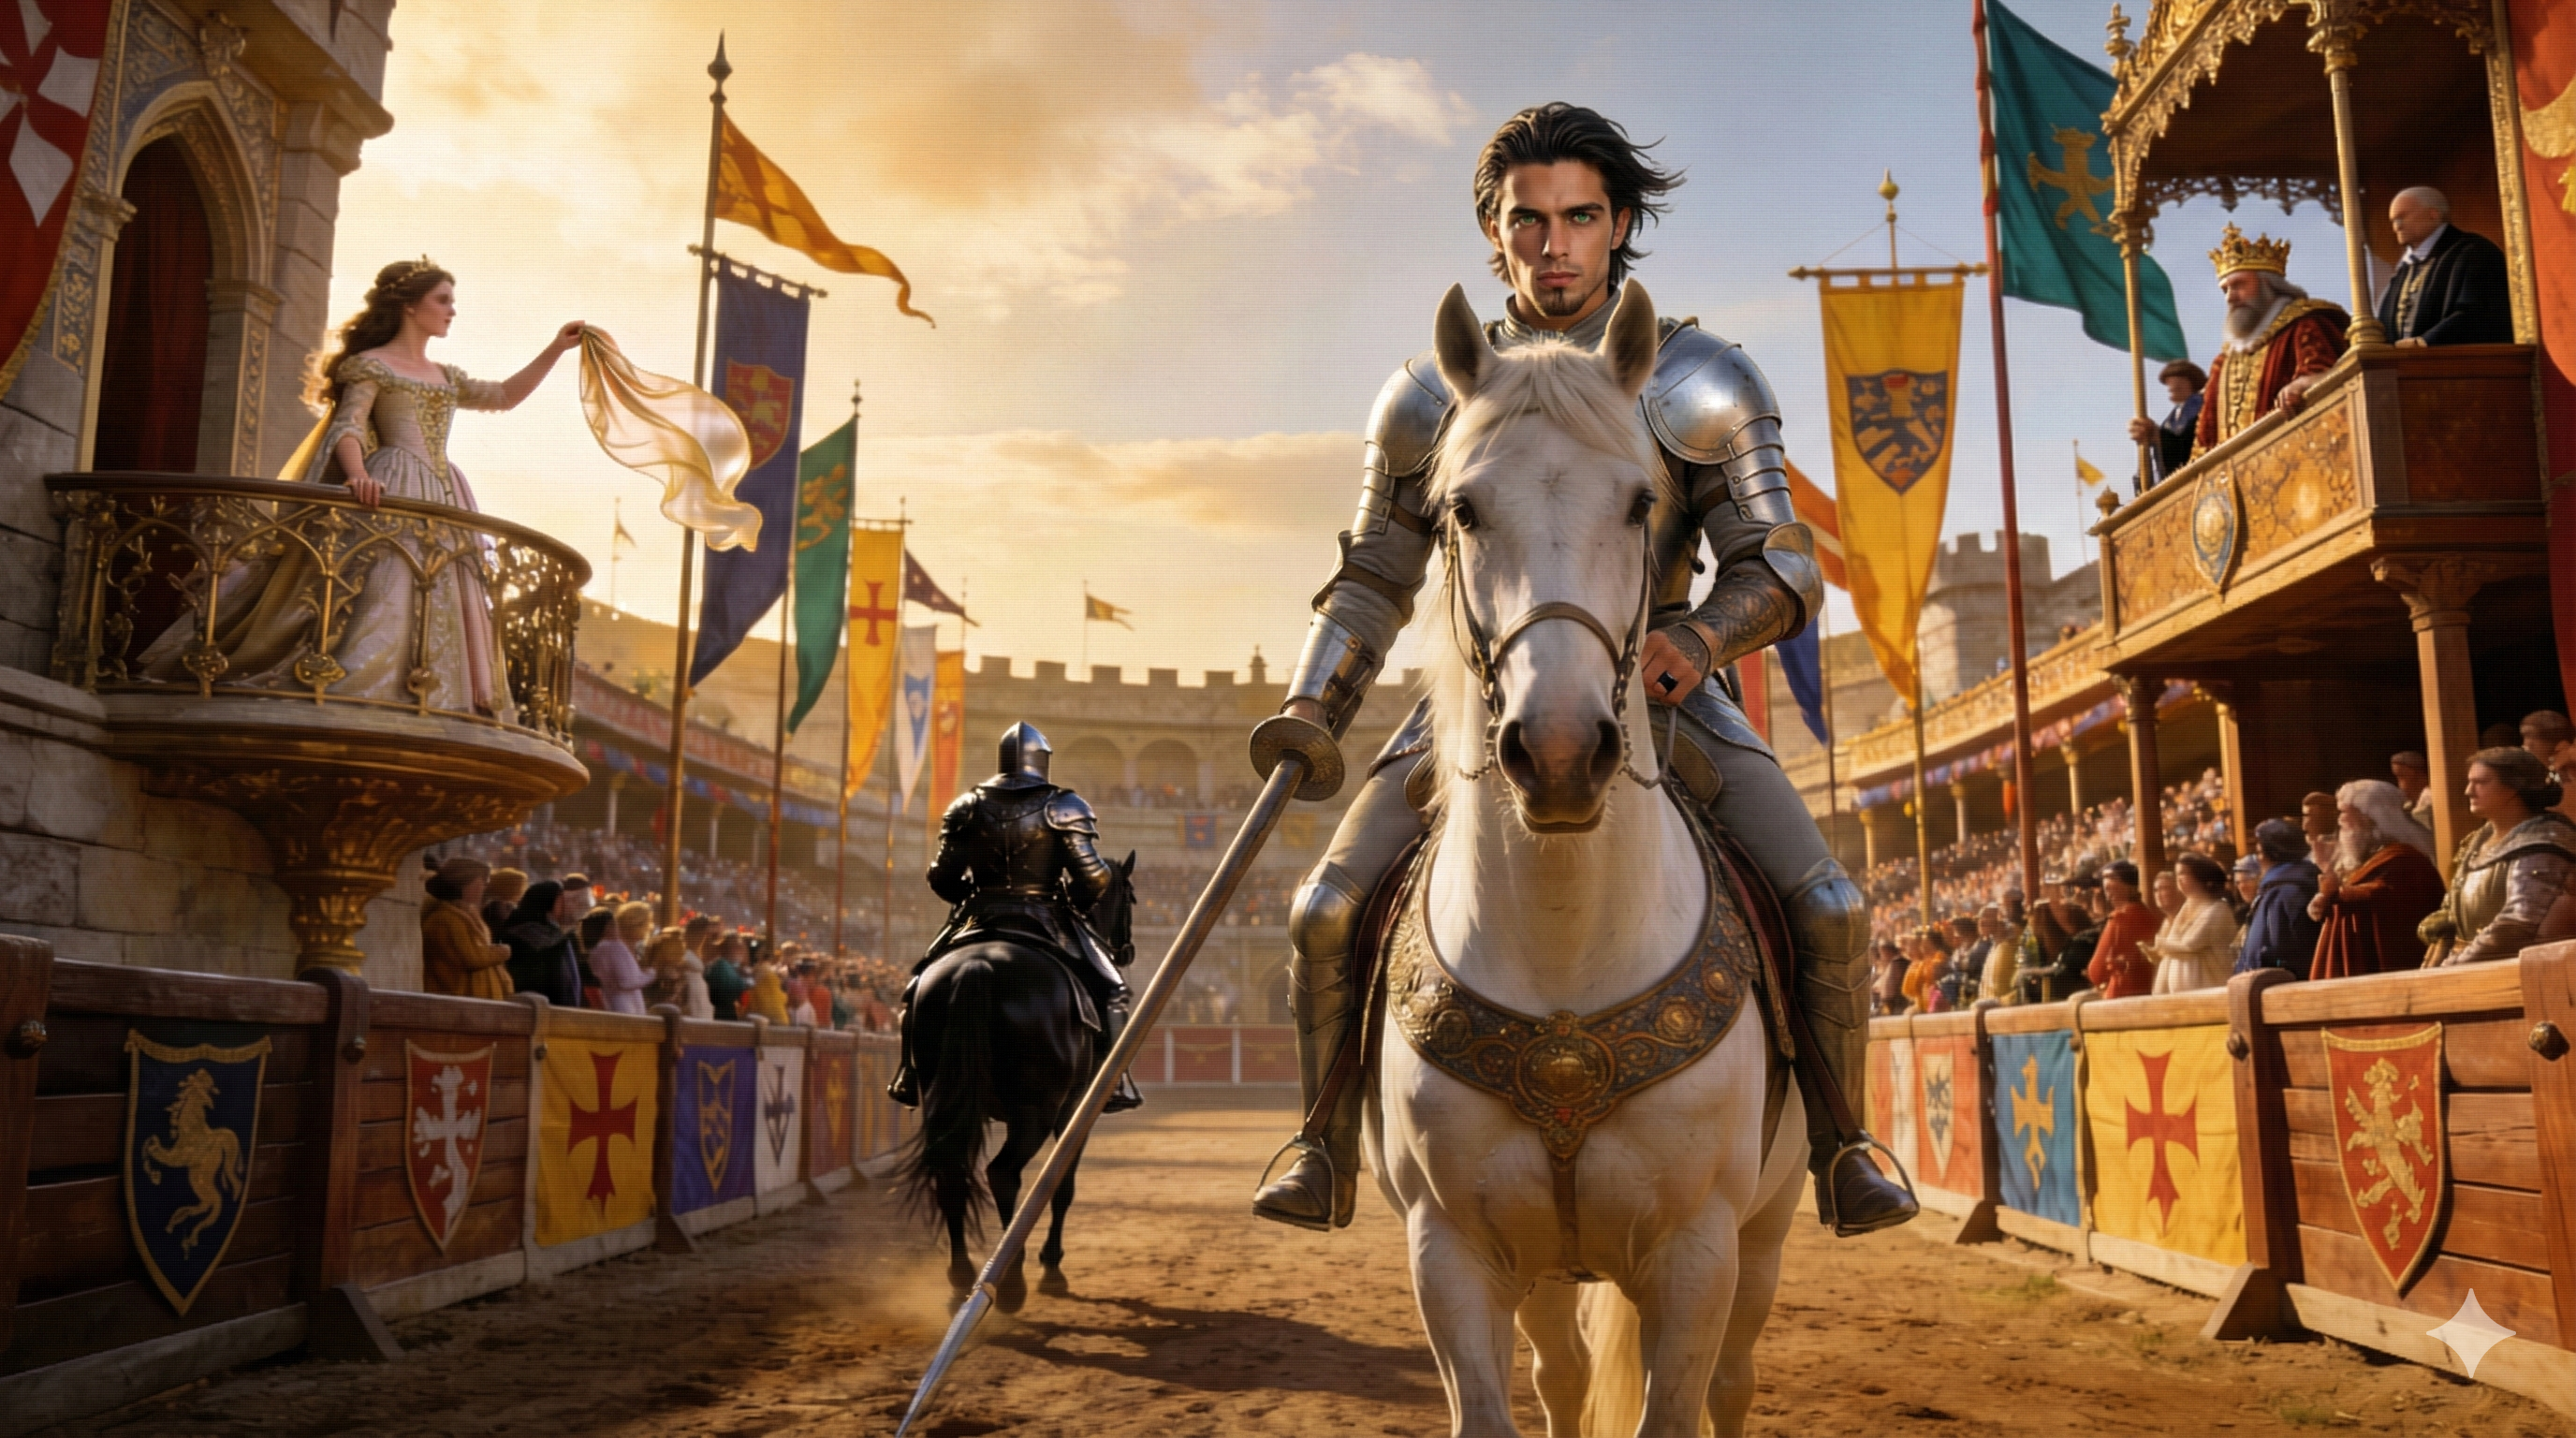
\includegraphics[width=\textwidth]{images/hero_in_backgrounds/medieval.png}
\end{center}

\column{0.4\textwidth}
\textbf{Story:} Hero becomes a jousting champion.

\vspace{0.3cm}
\textbf{Outfit:} Silver armor, no helmet

\vspace{0.3cm}
\textbf{Tools:}
\begin{itemize}
    \item Seedream: Tournament scene
    \item Nano Banana: Hero on horse
    \item Flux-2: Rearing pose edit
\end{itemize}
\end{columns}
\end{frame}

% ============================================
% SLIDE 7: Desert World
% ============================================
\begin{frame}{World 3: Desert — Journey}
\begin{columns}
\column{0.6\textwidth}
\begin{center}
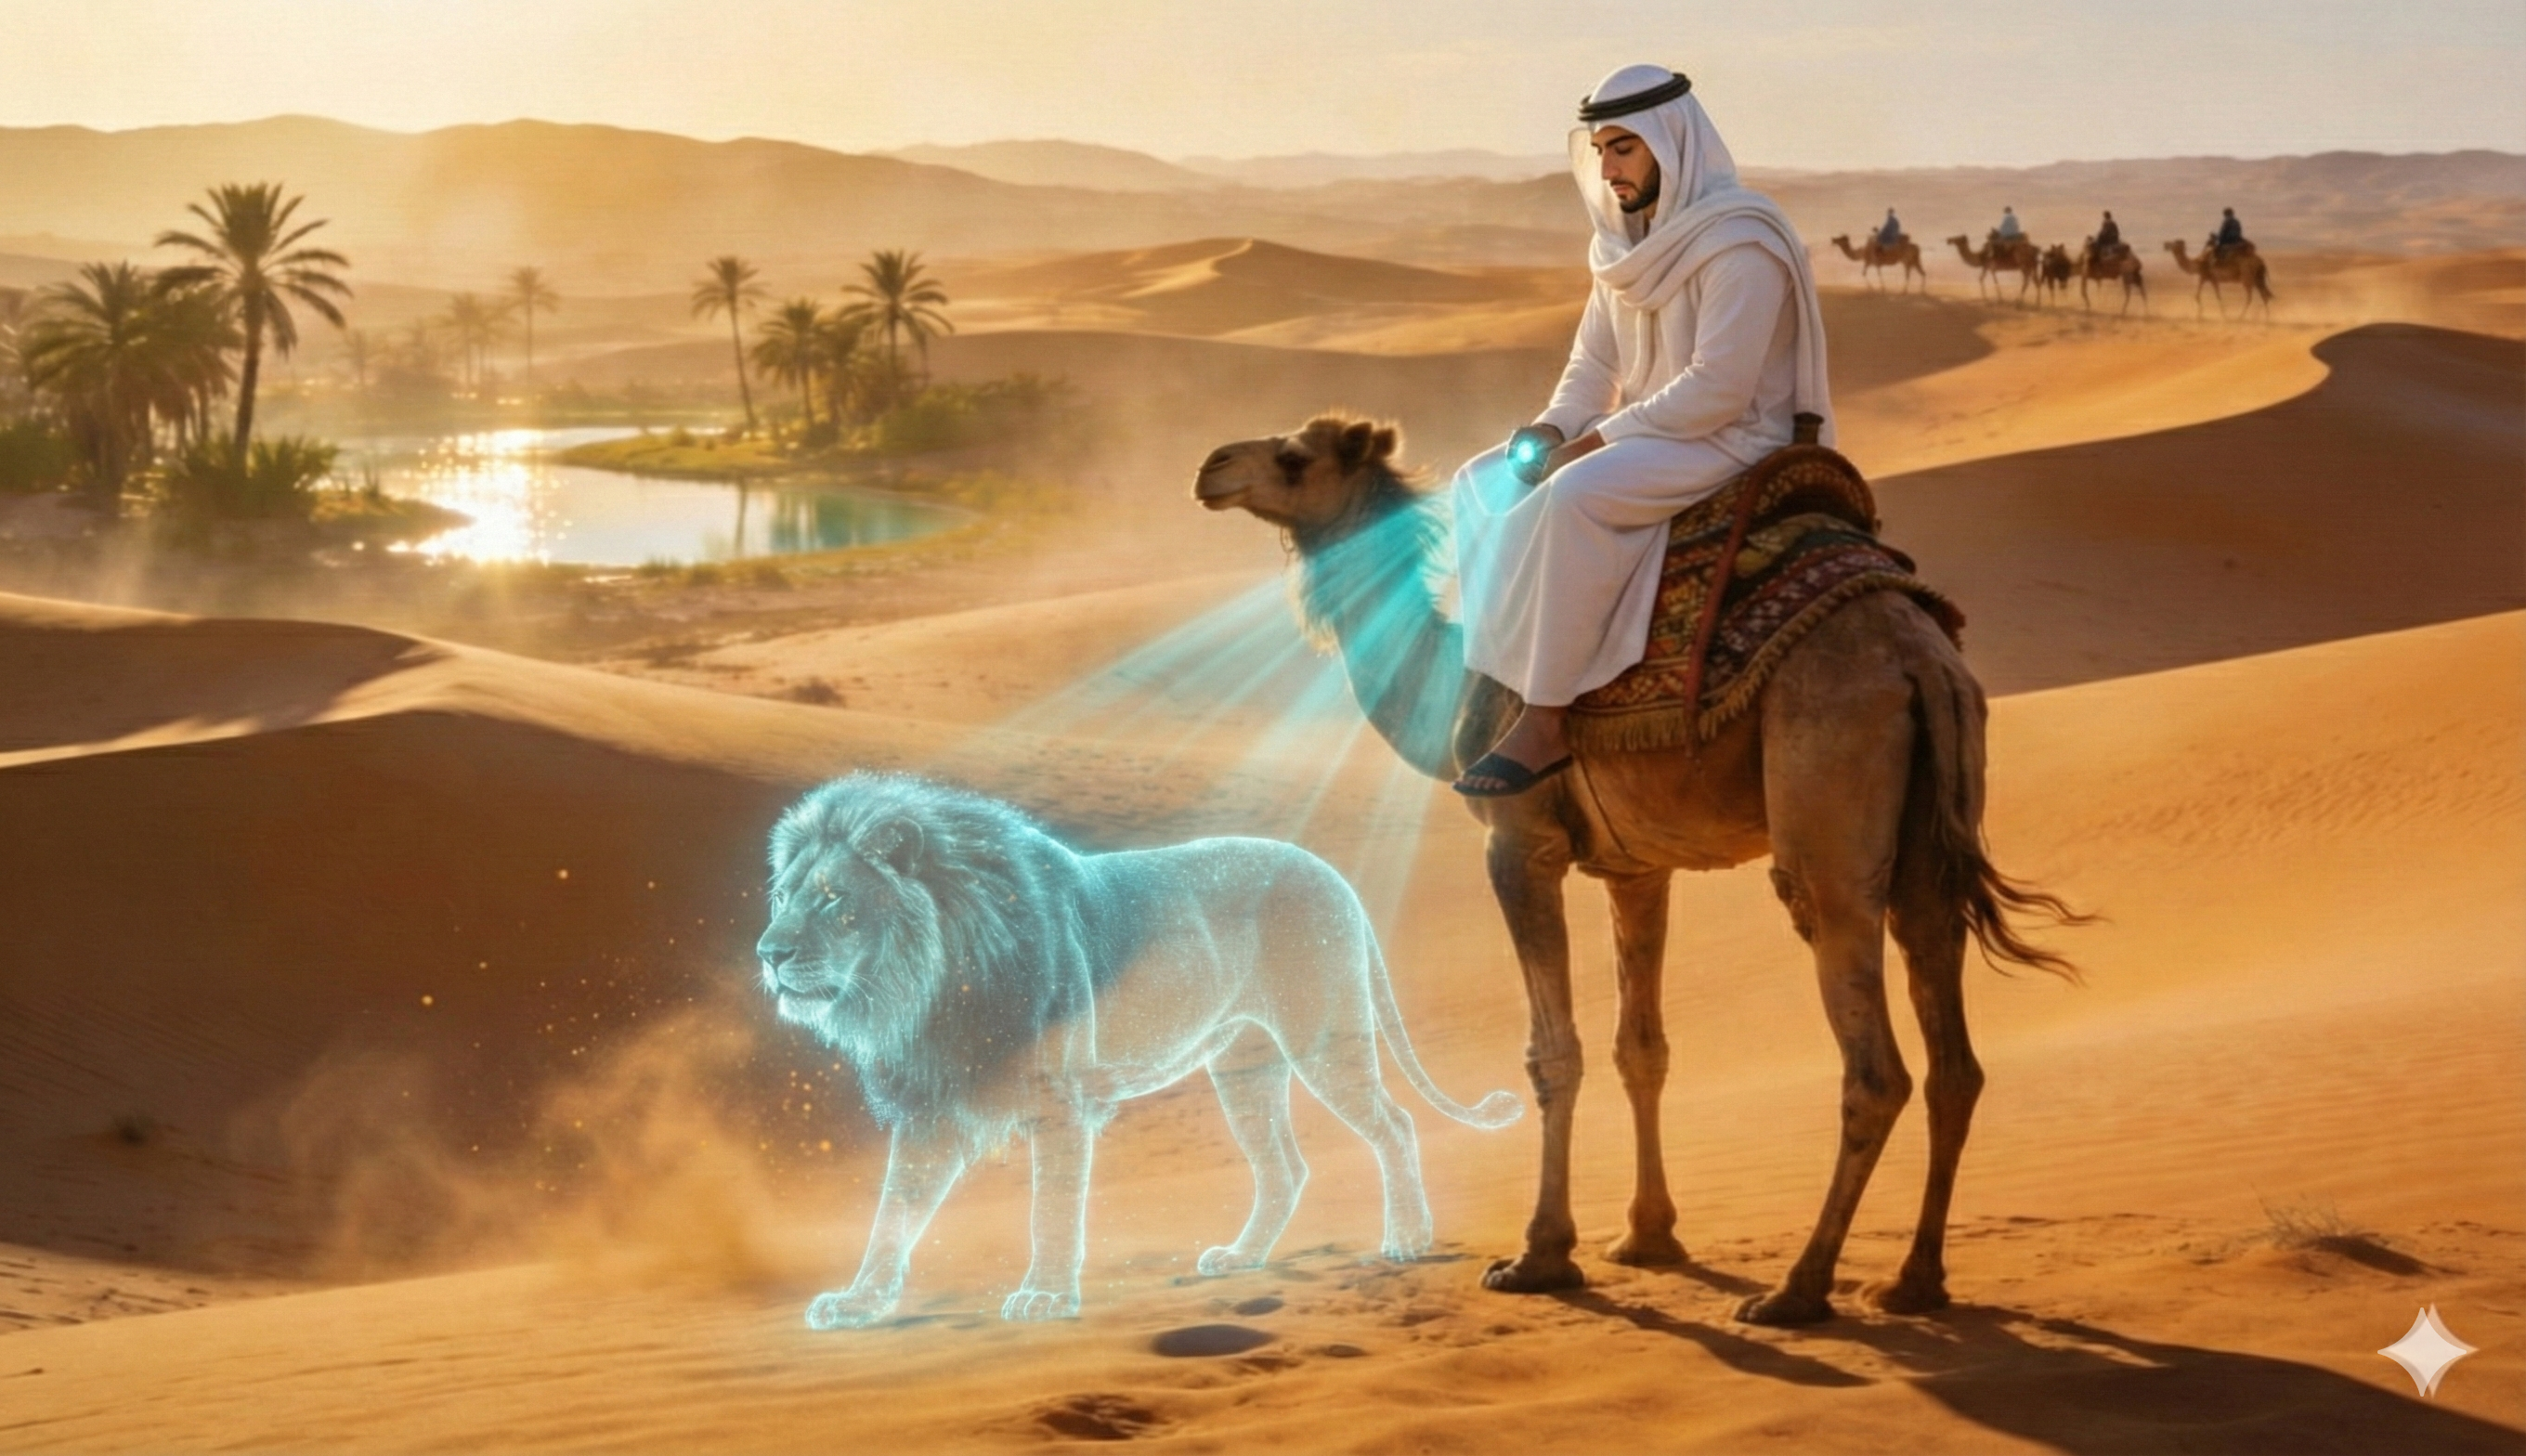
\includegraphics[width=\textwidth]{images/hero_in_backgrounds/desert.png}
\end{center}

\column{0.4\textwidth}
\textbf{Story:} Traveling through hostile lands with spirit companion.

\vspace{0.3cm}
\textbf{Outfit:} White desert robes, keffiyeh

\vspace{0.3cm}
\textbf{Tools:}
\begin{itemize}
    \item Seedream: Desert oasis
    \item Nano Banana: Hero on camel
\end{itemize}
\end{columns}
\end{frame}

% ============================================
% SLIDE 8: Cyberpunk World
% ============================================
\begin{frame}{World 4: Cyberpunk — Future Memories}
\begin{columns}
\column{0.6\textwidth}
\begin{center}
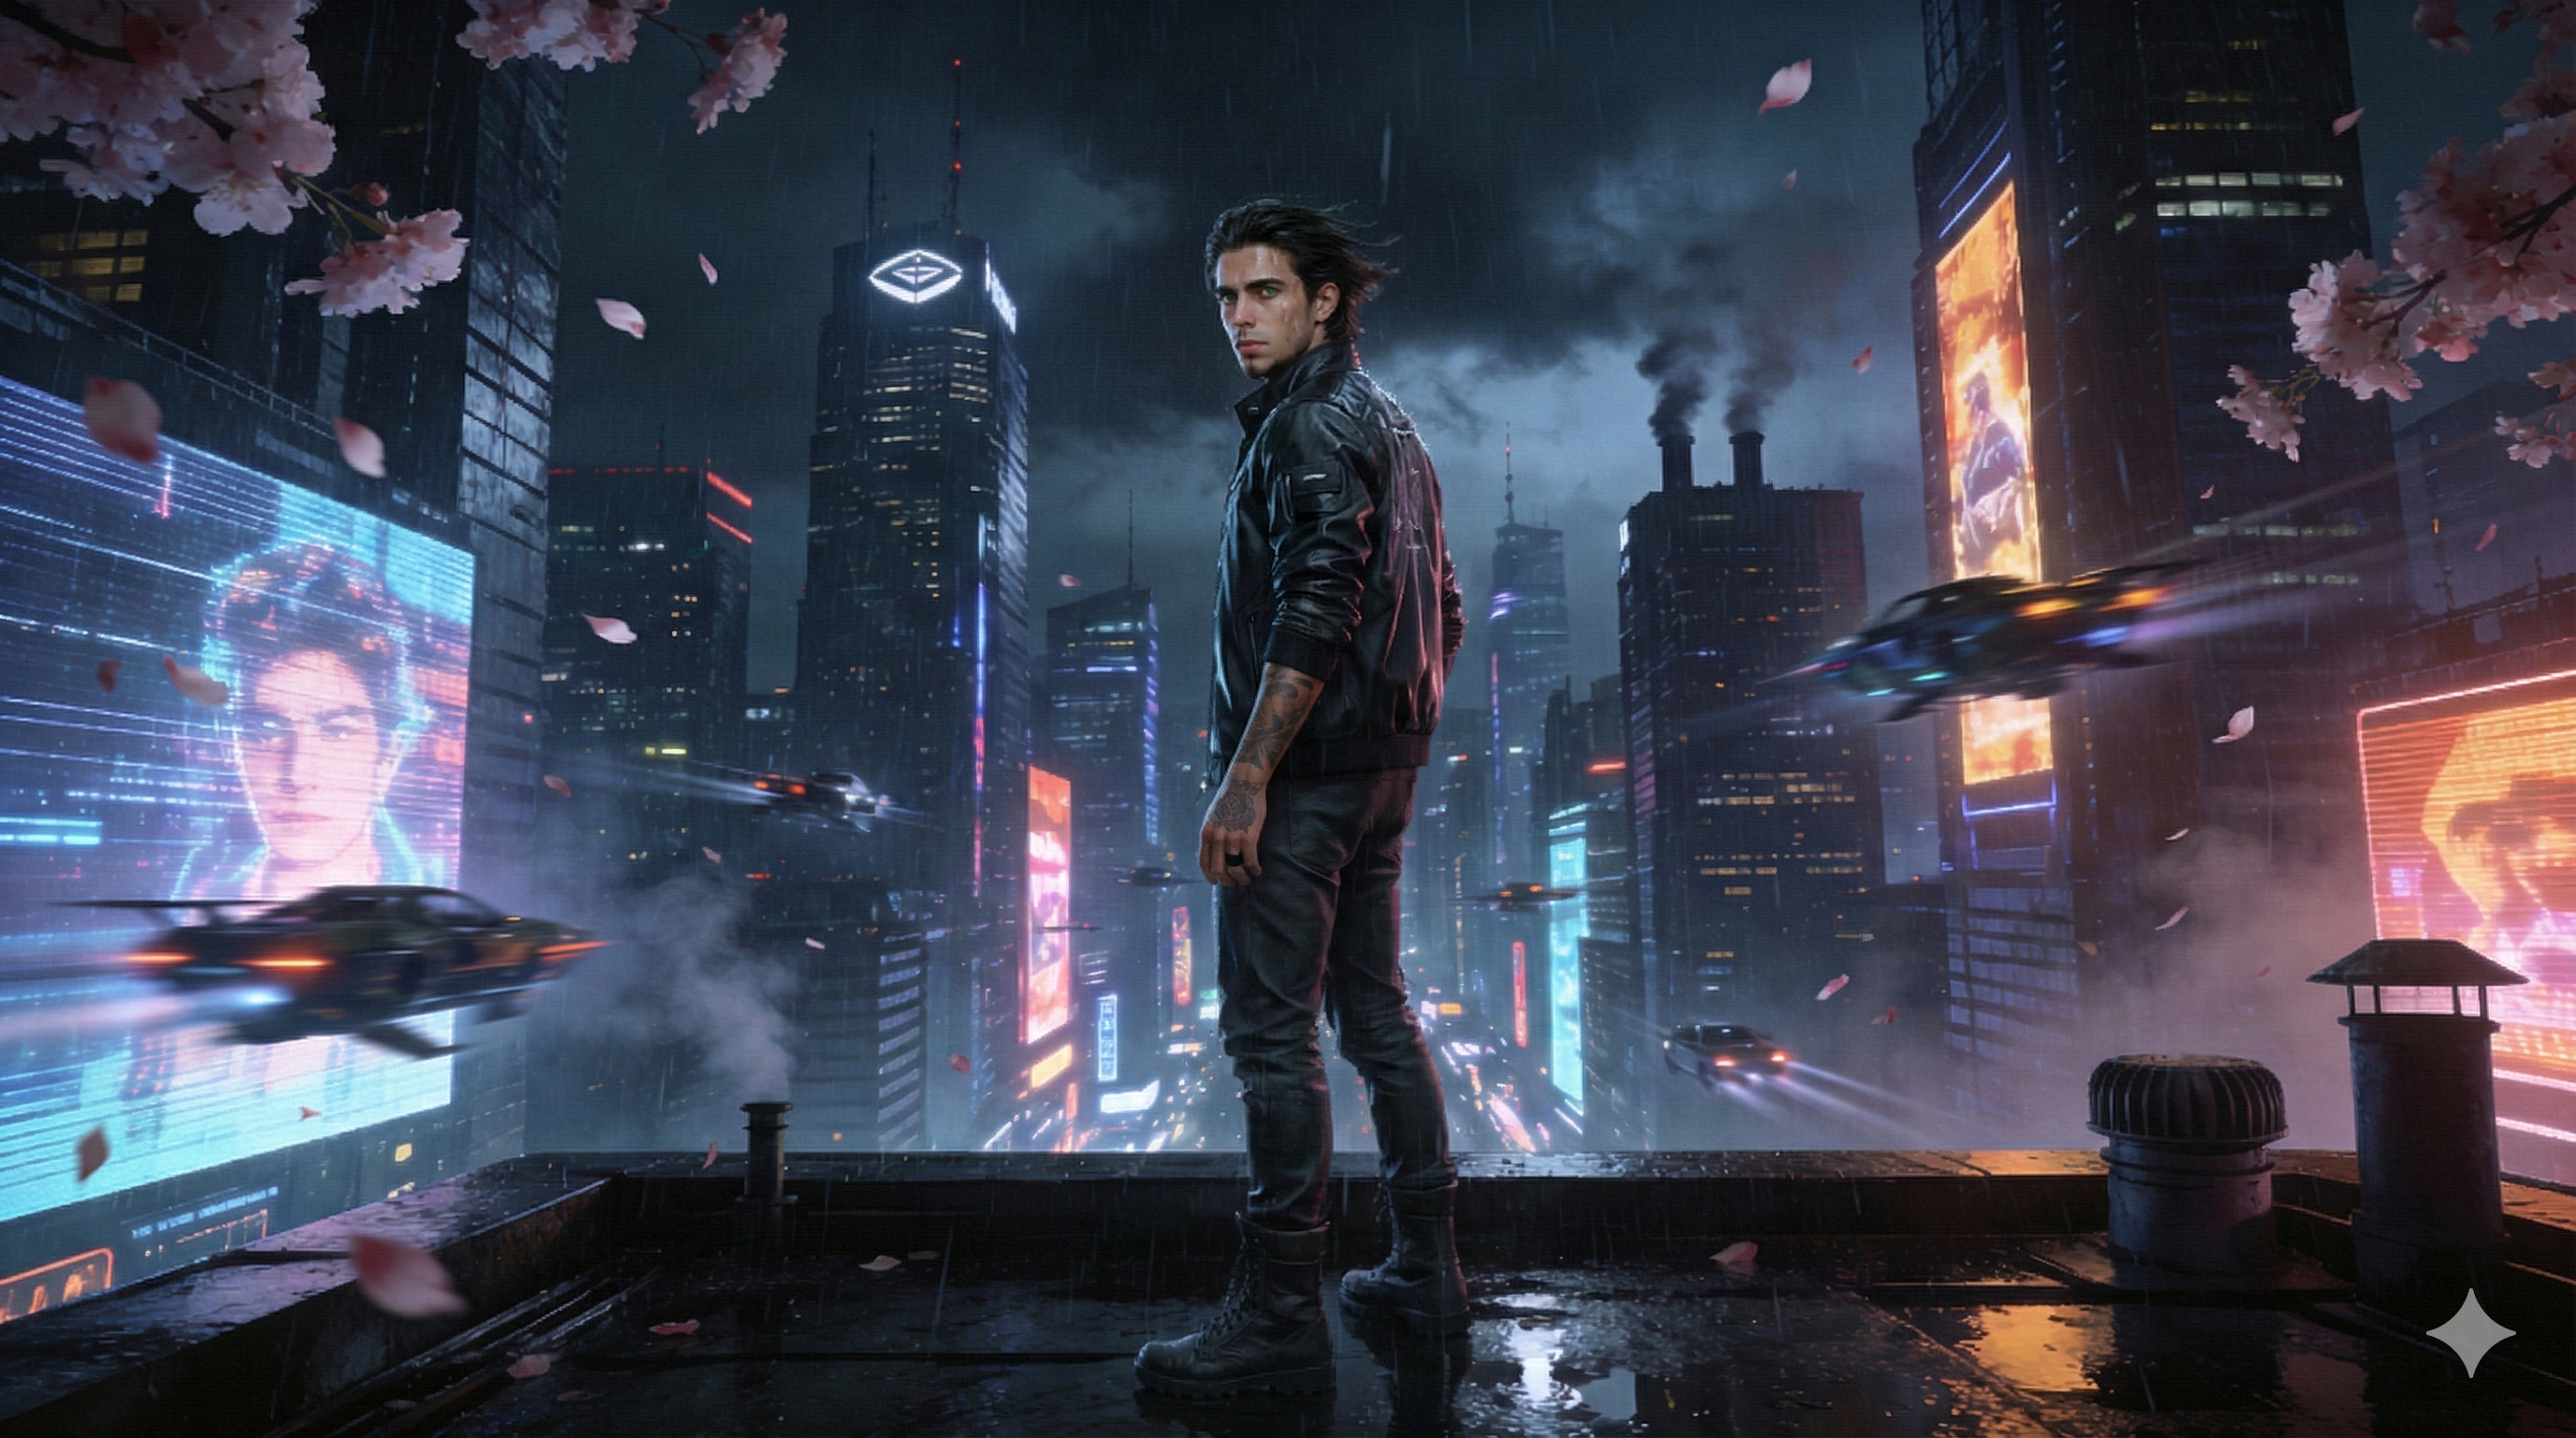
\includegraphics[width=\textwidth]{images/hero_in_backgrounds/cyberpunk.png}
\end{center}

\column{0.4\textwidth}
\textbf{Story:} Hero remembers the lion as a hologram from his ring.

\vspace{0.3cm}
\textbf{Outfit:} Futuristic tech jacket

\vspace{0.3cm}
\textbf{Tools:}
\begin{itemize}
    \item Seedream: Neon city
    \item Nano Banana: Hero insert
    \item Flux-2: Hologram edit
\end{itemize}
\end{columns}
\end{frame}

% ============================================
% SLIDE 9: In-Context Editing Comparison
% ============================================
\begin{frame}{In-Context Editing: Flux-2 vs Nano Banana}
\begin{columns}
\column{0.5\textwidth}
\begin{center}
\textbf{Flux-2 Pro}\\
\includegraphics[width=0.8\textwidth]{images/in-context-editing/flux-2/medieval.jpg}\\
\small Crisp, detailed, creative
\end{center}

\column{0.5\textwidth}
\begin{center}
\textbf{Nano Banana}\\
\includegraphics[width=0.8\textwidth]{images/in-context-editing/nano-banana/medieval.png}\\
\small Logical, slight quality drop
\end{center}
\end{columns}

\vspace{0.3cm}
\begin{center}
\textbf{Winner: Flux-2 Pro} — Better quality, but both can alter character identity
\end{center}
\end{frame}

% ============================================
% SLIDE 10: Conclusions
% ============================================
\begin{frame}{Conclusions \& Lessons Learned}
\begin{columns}
\column{0.5\textwidth}
\textbf{Key Lessons:}
\begin{itemize}
    \item Start with best generation tool (Seedream)
    \item Design ``hero spots'' in backgrounds
    \item Simpler edits = better consistency
    \item Use explicit constraints in prompts
\end{itemize}

\vspace{0.3cm}
\textbf{Challenges:}
\begin{itemize}
    \item Character identity changes in complex edits
    \item Quality reduction in Nano Banana
\end{itemize}

\column{0.5\textwidth}
\textbf{Best Practices:}
\begin{itemize}
    \item Create reference sheets first
    \item Test in multiple tools
    \item Use ``DO NOT MODIFY'' constraints
\end{itemize}

\vspace{0.3cm}
\begin{center}
\Large\textbf{Thank You!}\\
\normalsize Questions?
\end{center}
\end{columns}
\end{frame}

\end{document}
